\section{Thuật toán Tìm kiếm bằng Ô-tô-mát (Automaton)}

\subsection{Đặc điểm chính}

Thuật toán Tìm kiếm bằng Ô-tô-mát sử dụng một ô-tô-mát hữu hạn tất định
(DFA) được xây dựng từ mẫu $x$ để duyệt văn bản $y$ chỉ trong một lượt,
không cần quay lui. Đây là một trong những thuật toán tìm kiếm xâu hiệu
quả nhất về số lần kiểm tra ký tự trong pha tìm kiếm. Các đặc điểm nổi
bật của thuật toán bao gồm:

\begin{itemize}
    \item Pha tiền xử lý xây dựng ô-tô-mát $\mathcal{A}(x)$ trong thời gian
          $O(m + |\Sigma|)$ và không gian $O(m \cdot |\Sigma|)$.
    \item Pha tìm kiếm có độ phức tạp thời gian $O(n)$ nếu ô-tô-mát được
          lưu trong bảng truy cập trực tiếp; $O(n \log |\Sigma|)$ trong
          trường hợp ngược lại.
    \item Thực hiện đúng $n$ lần kiểm tra ký tự văn bản trong pha tìm kiếm.
\end{itemize}

\subsection{Mô tả thuật toán}

Tìm kiếm xâu $x$ bằng ô-tô-mát bắt đầu bằng việc xây dựng ô-tô-mát hữu
hạn tất định tối thiểu (DFA) $\mathcal{A}(x)$ nhận dạng ngôn ngữ
$\Sigma^{*}x$. Ô-tô-mát này được định nghĩa là bộ bốn thành phần
$\mathcal{A}(x) = (Q,\, q_0,\, T,\, E)$, trong đó:

\begin{itemize}
    \item $Q$ là tập các trạng thái, được đánh nhãn theo độ dài tiền tố
          tương ứng, từ $0$ đến $m$.
    \item $q_0$ là trạng thái khởi đầu.
    \item $T$ là tập các trạng thái kết thúc (terminal).
    \item $E$ là tập các chuyển trạng thái; các chuyển còn thiếu đều dẫn
          về trạng thái khởi đầu $0$.
\end{itemize}

Sau khi xây dựng xong $\mathcal{A}(x)$, pha tìm kiếm hoạt động như sau:
văn bản $y$ được phân tích tuần tự bằng $\mathcal{A}(x)$, bắt đầu từ
trạng thái khởi đầu $q_0$. Mỗi khi trạng thái kết thúc được đạt tới,
một lần xuất hiện của $x$ trong $y$ được ghi nhận.

\subsection{Cài đặt bằng C++}

\begin{verbatim}
#include <iostream>
#include <vector>
#include <string>
#include <cstring>
using namespace std;

const int ASIZE = 256;

// Xây dựng bảng chuyển trạng thái của DFA
// aut[s][c] = trạng thái tiếp theo từ trạng thái s với ký tự c
void preAut(const string& x, int m,
            vector<vector<int>>& aut) {
    for (int i = 0; i < m; ++i) {
        // Sao chép chuyển trạng thái từ trạng thái hiện tại
        for (int c = 0; c < ASIZE; ++c)
            aut[i + 1][c] = aut[i][c];
        // Thiết lập chuyển đúng theo ký tự mẫu
        aut[i + 1][(unsigned char)x[i]] = i + 1;
        // Sửa lại các chuyển không khớp dựa trên hàm thất bại
        // (đã được mã hóa ngầm trong quá trình sao chép)
    }
}

// Tìm tất cả vị trí xuất hiện của x trong y
vector<int> AUT(const string& x, const string& y) {
    int m = (int)x.size();
    int n = (int)y.size();
    vector<int> results;

    // Khởi tạo bảng chuyển trạng thái kích thước (m+1) x ASIZE
    vector<vector<int>> aut(m + 1, vector<int>(ASIZE, 0));

    /* Preprocessing */
    preAut(x, m, aut);

    /* Searching */
    int state = 0;
    for (int j = 0; j < n; ++j) {
        state = aut[state][(unsigned char)y[j]];
        if (state == m)
            results.push_back(j - m + 1); // OUTPUT
    }

    return results;
}

int main() {
    string y = "ababcabcabababd";
    string x = "abab";

    vector<int> pos = AUT(x, y);

    cout << "Vi tri xuat hien: ";
    for (int p : pos)
        cout << p << " ";
    cout << endl;

    return 0;
}
\end{verbatim}

\subsection{Kiểm nghiệm thuật toán}

Giả sử ta có mẫu $x = \texttt{abab}$ và văn bản
$y = \texttt{ababcabcabababd}$. Ô-tô-mát $\mathcal{A}(x)$ được xây dựng
với $m + 1 = 5$ trạng thái, đánh số từ $0$ đến $4$, trong đó trạng thái
$4$ là trạng thái kết thúc. Pha tìm kiếm duyệt qua từng ký tự của $y$,
chuyển trạng thái theo bảng $\mathcal{A}(x)$ và ghi nhận vị trí khớp mỗi
khi đạt trạng thái kết thúc.

\begin{figure}[H]
    \centering
    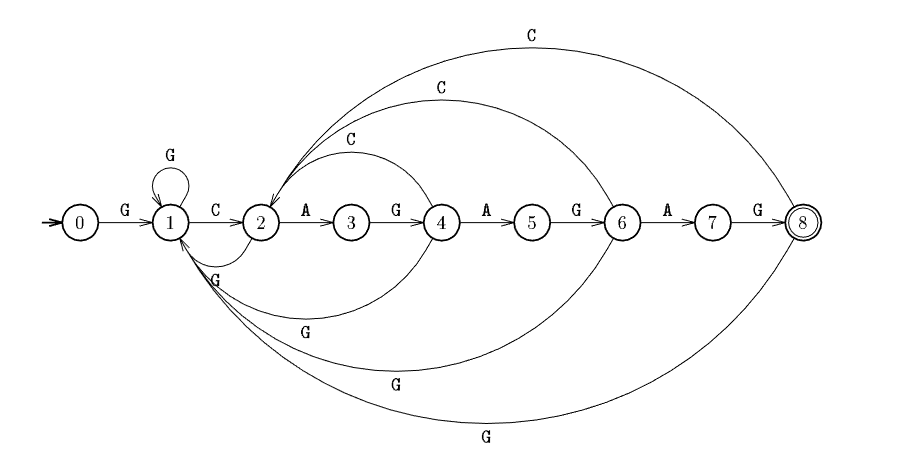
\includegraphics[width=15cm]{Images/2026-05-15-11-10-25.png}
    \caption{Minh họa ô-tô-mát DFA của mẫu x trong thuật toán Automaton}
    \label{fig:finite-automaton-dfa}
\end{figure}

Các trạng thái được đánh nhãn theo độ dài của tiền tố mà chúng đại diện. 
Các chuyển trạng thái không được định nghĩa đều dẫn về trạng thái khởi đầu 0.

\textbf{Pha tìm kiếm}

Trạng thái bắt đầu là 0.


\begin{figure}[H]
    \centering
    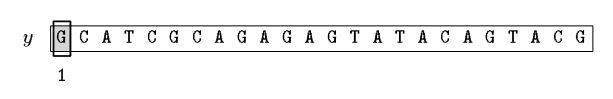
\includegraphics[width=10cm]{Images/2026-05-15-11-19-34.png}
    \caption{Bước 1 trong quá trình thực hiện thuật toán Automaton}
    \label{fig:finite-automaton-step-1}
\end{figure}

\begin{figure}[H]
    \centering
    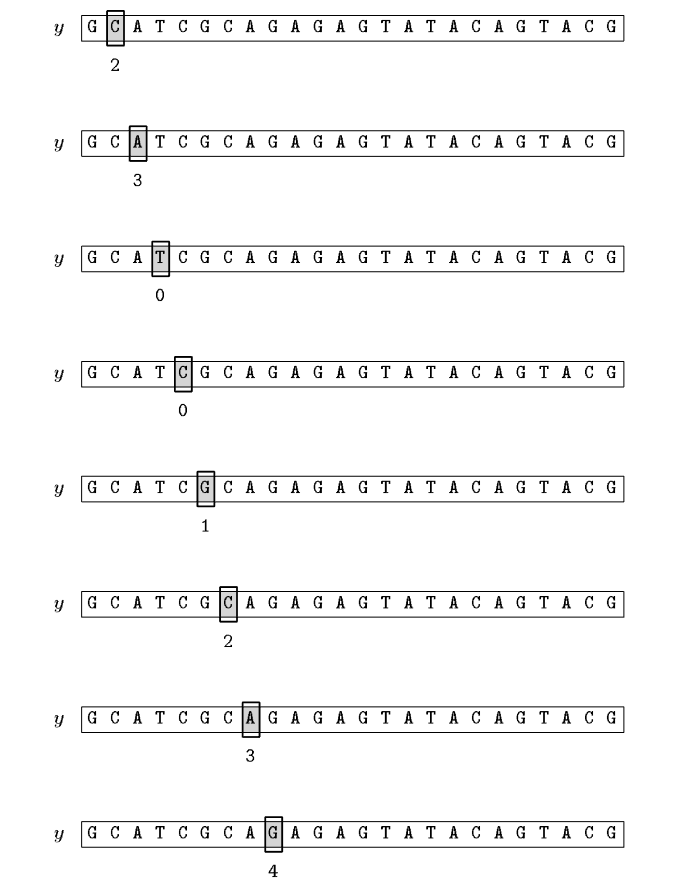
\includegraphics[width=10cm]{Images/2026-05-15-11-19-59.png}
    \caption{Bước 2 trong quá trình thực hiện thuật toán Automaton}
    \label{fig:finite-automaton-step-2}
\end{figure}

\begin{figure}[H]
    \centering
    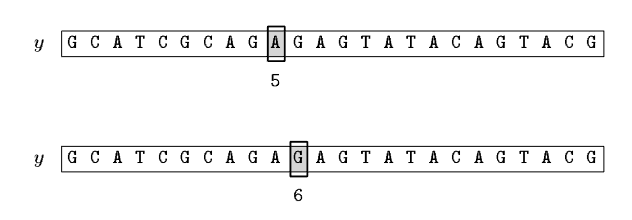
\includegraphics[width=10cm]{Images/2026-05-15-11-20-20.png}
    \caption{Bước 3 trong quá trình thực hiện thuật toán Automaton}
    \label{fig:finite-automaton-step-3}
\end{figure}

\begin{figure}[H]
    \centering
    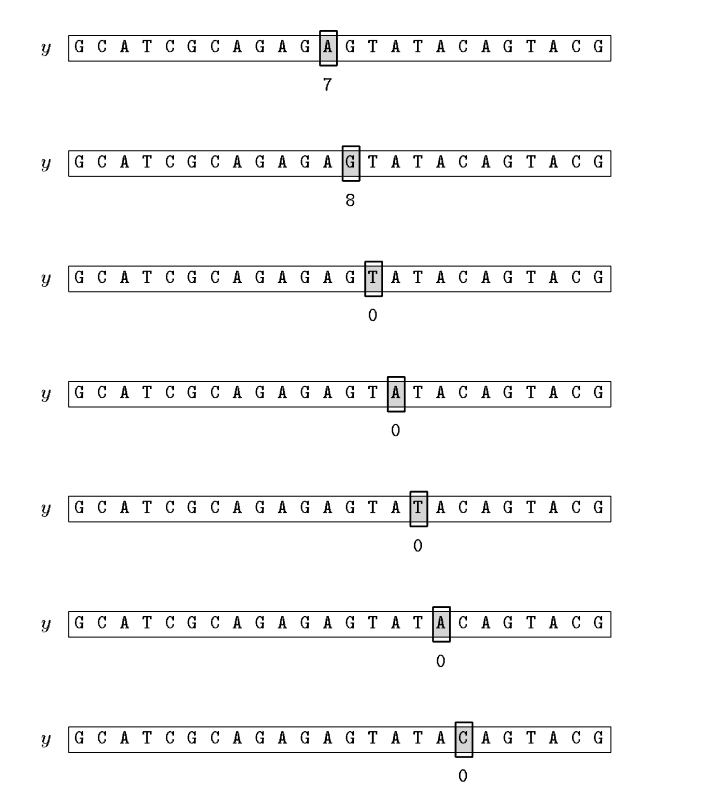
\includegraphics[width=10cm]{Images/2026-05-15-11-20-41.png}
    \caption{Bước 4 trong quá trình thực hiện thuật toán Automaton}
    \label{fig:finite-automaton-step-4}
\end{figure}

\begin{figure}[H]
    \centering
    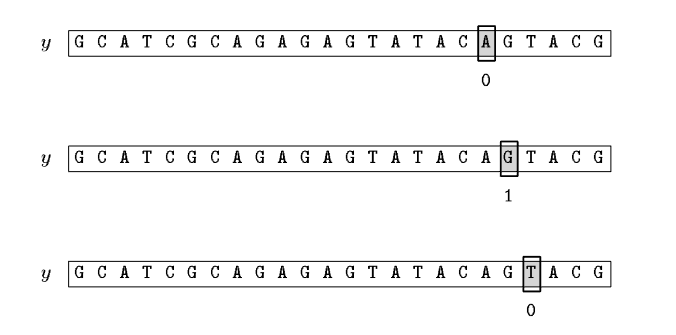
\includegraphics[width=10cm]{Images/2026-05-15-11-21-00.png}
    \caption{Bước 5 trong quá trình thực hiện thuật toán Automaton}
    \label{fig:finite-automaton-step-5}
\end{figure}

\begin{figure}[H]
    \centering
    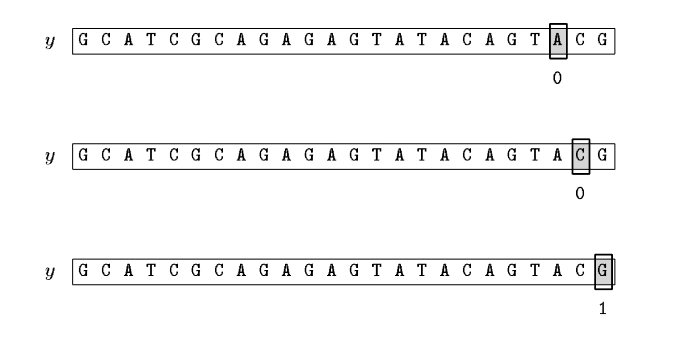
\includegraphics[width=10cm]{Images/2026-05-15-11-21-16.png}
    \caption{Bước 6 trong quá trình thực hiện thuật toán Automaton}
    \label{fig:finite-automaton-step-6}
\end{figure}

Thuật toán sử dụng 24 phép so sánh chuỗi trong ví dụ trên.